%%%%%%%%%%%%%%%%%%%%%%%%%%%%%%%%%%%%%%%%%%%%%%%%%%%%%%%%%%%%%%%%%%%%%%%%%%%%%%%%
% experiment.tex: Chapter describing the experiment
%%%%%%%%%%%%%%%%%%%%%%%%%%%%%%%%%%%%%%%%%%%%%%%%%%%%%%%%%%%%%%%%%%%%%%%%%%%%%%%%
\chapter{Hadron Collider and Detector}
This section describes the particle accelerator and detectors that are used to produced and detect particles at colliders. The first section describes the particle accelerator while the following section describes the CMS detectors with emphasis to those sections which are directly relevant to this analysis. A detailed description of the LHC and detectors can be found in \cite{LHC} and \cite{CMSD}.
\section{Large Hadron Collider}
\subsection{Overview}
The Large Hadron collider~(LHC) is a proton-proton and heavy ion collider designed to achieve a center of mass $\displaystyle{\sqrt{S}}$ energy of 14~TeV. It is hosted and controlled by the European Organisation for Nuclear Research~(CERN). Unlike linear colliders, the LHC is a circular collider with nearly 27~km in circumference located at the border between France and Switzerland. It is designed to smash protons and ions against each other controlled by powerful magnets at officially four main locations. At each major collision point are multi-purpose particle detectors ranging from A Toroidal LHC Apparatus~(ATLAS) and Compact Muon Solenoid~(CMS) both non-fixed target detectors, A Large Ion Collider Experiment~(ALICE) for colliding heavy ions and finally Large Hadron Collider beauty~(LHCb), a fixed target experiment for investigating the properties of B-Hadrons. We  give a full description of the important parts of the LHC in the following subsections, detail discussion of other interesting parts can be found here \cite{LHC}.
There are three main steps prior to colliding protons or ions at the LHC.  The first is ramping up the energy of the beams followed by squeezing the beams at interaction points( CMS or ATLAS) and finally remove the separator bumps that are formed by local corrector magnets.
Thus our description of the LHC will follow this three stages.
\begin{center}
\centering
\mbox{
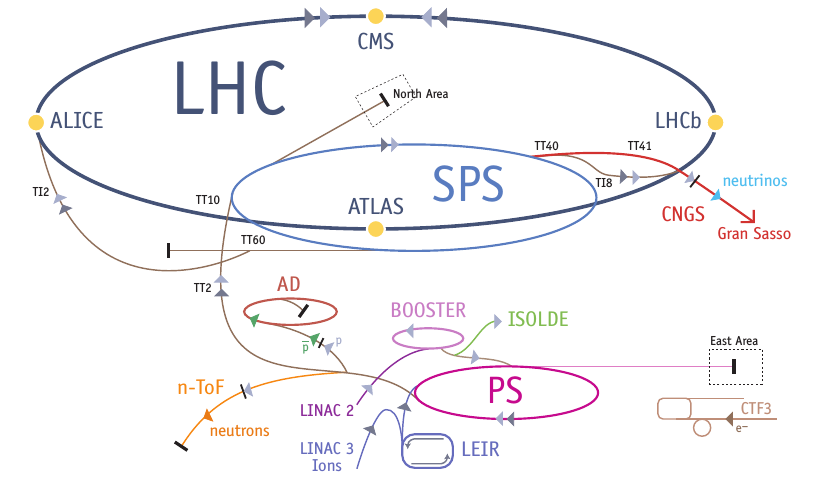
\includegraphics[width=6in]{THESISPLOTS/The_LHC.png}}
\captionof{figure}{Schematic diagram showing the full Large hadron Collider. Image taken from \cite{LHCB}}
\label{fig:LHC}
\end{center}
\subsection{Colliding Energy}
Hydrogen gas is inserted into a linear accelerator called Linac2 where they are stripped off of their orbiting electrons to become hydrogen ions or protons. Under the influence of electric fields, these protons are accelerated to an energy of 50~\MeV creating a stream of particles called \textit{particle beams}. These beams are arranged in packets known as \textit{bunches}. Particle acceleration if provided through the use of Radio-Frequency~(RF) cavities containing electromagnetic fields which oscillate at a particular frequency. The protons surf this electromagnetic fields and are group in troughs of the electromagnetic waves called RF~\textit{buckets}. The circular nature of the synchrotron accelerator ensures that the protons pass many times through a cavity and during each time their energy can be slowly increase to reach the design energy.
The 50~\MeV protons from the Linac2 are injected into the proton synchrotron Booster~(PSB). The PSB accelerates the protons to up to 1.4~\GeV and inject them into the Proton Synchrotron~(PS) which pushes the protons energy to 25~\GeV. These protons travelling at 99.93\% the speed of light are sent to the Super Proton Synchrotron~(SPS) and accelerated to an energy of 450~\GeV. They are finally transferred into the LHC ring(both in a clockwise and anti-clockwise direction) and accelerated for about 20 minutes to their norminal energy of 7~\TeV. As this point these protons are travelling with the speed of 99.9999\% the speed of light. Powerful magnets are used to keep the beeps travelling in the circular LHC ring. The advantage of circular particle colliders such as the LHC over fix target colliders is that, the energy available to make new particles called the center of mass energy denoted as $\sqrt{S}$ is simply the sum of the energy of the two beams i.e $\sqrt{S} = \mathit{E}_{\mbox{beam1}} +   \mathit{E}_{\mbox{beam2}}$ compared to $\sqrt{\mathit{E}_{\mbox{beam}}}$ for fix target experiments. In the case of the LHC, each beam is designed to have energy of 7~\TeV and that makes $\sqrt{S} = 14$~\TeV. Although in circular collider, an accelerating charge particles like the proton would loose energy in for the form of radiation which is inversely proportional to the mass of the charge particle to the fourth power requiring  the need for continuous addition of energy after each turn to maintain the beam energy to a stable value. Since the proton's mass is  about $0.938$~\GeV which is close to 1~\GeV, this lost of energy is not very significant unlike  electrons  whose mass of about $0.000511$~\GeV making their energy lose through radiation more and thus less preferable to use as the main particles for a circular hadron collider. However, the debris of particles produced when electrons collide is much less compared to that of hadrons making analysis in a hadron collider more challenging. 
\subsection{Luminosity}
Luminosity is the measurement of the number of collisions that can be produced in a collider per squared area per second. This is known as the instantaneous luminosity and it is related to the cross-section(a probabilistic measure of the possibility of a given collision process happening) through the equation:

\begin{equation}
N_{\mbox{events/sec}} = \mbox{Luminosity} \cdot \mbox{Cross Section}
\end{equation}
where the luminosity $\mathscr{L}$ is related to the total integrated luminosity(delivered luminosity over time) $\mathrm{L} = \int \mathscr{L}dt$ and is defined in terms of accelerator(assuming round beams and equal values of beta function) parameters as:
\begin{equation}\label{lumi}
\mathscr{L} = \frac{1}{4\pi}\cdot\left(f_{rev}\mathit{n}_{b}\mathit{N}_{b}\right)\cdot\frac{\mathit{N}_{b}}{\varepsilon_{N}}\cdot \frac{\gamma}{\beta^{\ast}}\cdot \mathscr{R}(\theta_{c},\varepsilon,\beta^{\ast},\sigma_{z} )
\end{equation}

where $\mathit{N}_{b}$ is the number of particles per bunch, $\mathit{n}_{b}$ is the number of bunches, $f_{rev}$ is the revolutionary frequency, $\gamma = E/m_{p}$ is the relativistic factor, $\varepsilon_{N}$ is the normalised beam emittance which along with $\beta^{\ast}$, the value of the amplitude or beta function at interaction point, determines the size of the beam. $\mathscr{R}$ is the geometrical reduction factor arising from the fact that the beams to not collide head-on but at a non-zero angle called the crossing angle or \textit{"Piwinski angle"}( $\phi \equiv \frac{\theta_{c}\sigma_{z}}{2\sigma_{x}}$). This effect is known as the \textit{hour-glass effect}.
From the above definition \eqref{lumi}, it is evident that keeping the emittance (meaning particles in beam are confined to a small distance and have nearly the same momentum ) means the likelihood of particle interaction will be greater and thus higher luminosity. However this is often not easy to archive as increasing the beam energy means reducing the beam emittance. The normalized emittance $\varepsilon_{N}$ is often used as its dependence on beam energy is a squared root dependence.
In the same way, lower beta values implies the width of beam is narrower or properly \textit{"squeezed"} at interaction point resulting to an increase in number of collisions hence higher luminosity.
This squeezing of depends on the quadruple magnet configuration and powering. 
In addition to low beam emittance and lowest value of beta function at interaction point($\beta^{\ast}$), one can also archive higher luminosity by using high population bunches($\mathit{N}_{b}$) and collide them at high frequency.
\paragraph*{Luminosity Measurement}\mbox{}\\
Obviously using equation \eqref{lumi} to determine the instantaneous and integrated luminosity would involve a lot of uncertainty in the measurements of about 20-30\%, as there are so many parameters whose value need to be measured precisely in a normal LHC operation. Rather specialised LHC runs known as \textit{"Van der Meer Scans"}\cite{lhclumi} are used to calibrate specialized equipments used for determining luminosity.
%The method employed by CMS(using TOTEM) is to use the total proton-proton~(\textit{p-p} cross section. 
The method employed by CMS is using the Hadronic Foward~(HF) calorimeter to make luminosity measurements.
Using production rates or cross sections of well and precisely calculable processes and rewriting \eqref{lumi} as:
\begin{equation}
 \mathscr{L} \equiv \frac{Rate_{tot}}{\sigma_{tot}}    = \frac{\mu \mathit{n}_{b} f_{rev}}{\sigma_{tot}} 
\end{equation}
where $\mu = \left\langle \mathit{N}_{tot}/ \mathit{n}_{b} \right\rangle $ is the \textit{average number of interactions per bunch crossing}.
CMS keeps track of "recorded" and "delivered" luminosity. Delivered luminosity refers to the luminosity delivered by LHC to CMS and one would expect this to be equal to  the amount recorded. However, there are instances where the CMS detector is unable to take data either because the data acquisition chain~(DAC) is busy or one of the CMS sub-detectors is temporarily down. Part of my job as a sub-detector expert during CMS data taking of LHC Run 1 was to make sure that the period of temporal unavailability of the ECAL sub-detector is as minimal as possible.
\begin{center}
\centering
\mbox{
%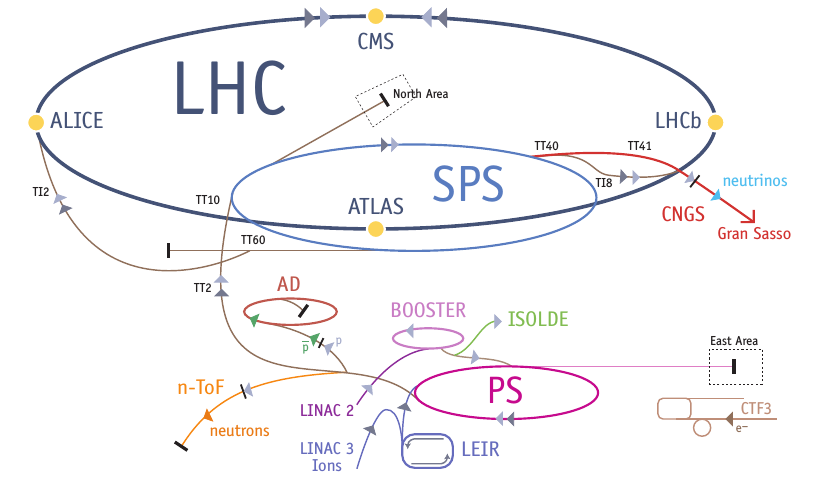
\includegraphics[width=6in]{THESISPLOTS/The_LHC.png}
}
\captionof{figure}{Recorded luminosity by CMS detector and LHC delivered luminosity in days/months during LHC Run 1 2012 operation.}
\label{fig:cmslumi}
\end{center}

  
%of well understood and calculable processes such as the production of $\mathrm{W}$ and $\mathrm{Z}$ bosons or di-leptons via  two photon exchange. 
\subsection{Superconducting Electromagnets}
The LHC design and operation uses a total of 9593 powerful magnets of different types for different purposes. Since there are two beams of protons running in clock-wise and anti-clock wise directions, the LHC uses an ingenious technique design  of the magnetic field in every dipole magnet generates a vector field $\mathbb{B}$ in each pipe pointing in opposite direction to that of the other but both always perpendicular to the beam directions. The Lorentz or magnetic force acting on the protons in both pipes always point towards the center thus keeping the beams in circular motion. In circular accelerators as the LHC and its smaller synchrotron rings, given the accelerator radius,$R$, the beam energy $p$ is determined by the strength $\mathbf{B}$ of the magnetic field. This can be easily understood using the Lorentz force  such that $\displaystyle{p[TeV] = 0.3\mathbf{B}[T]\cdot R[km] }$.
The LHC is is a 26.659~km in circumference machine using powerful dipole magnets with magnetic field strength of about 8.33~Tesla(T) are 7~TeV to keep the protons circulating in their curved path or orbits. The LHC operates using superfluid helium for heat transport at 1.4~K(-271.3~$^{\circ}C$)  temperature to prevent these near 1232 dipole magnets, 858 quadruple and 6208 correcting magnets from overheating due to the energy stored in these magnets. Conventional magnetics aren't convenient for modern particle accelerators with high center of mass energy for both performance and economic reason. Rather, superconducting magnets made with modern technology using  niobium-tantanium~(Nb-Ti) filaments strands or cables are used to provide the high magnetic field required. 
%These magnetics provide a magnetic field strength of about 8.33~T and are kept at about 1.4K in temperature during LHC operation.

Quadrupole electromagnet and correcting magnets are  used to keep the particles in the beam and archive the required focus and de-focusing needed. At interaction point, the quadrupole magnets are held symmetrically around the beam pipe to help squeeze the proton beams to very low values of beta function thus ensuring that many particle collisions as possible necessary for higher luminosity.


\subsection{Timing}
The Large Hadron Collider (LHC) is designed to collide proton-proton (pp) bunches every  24.95~ns at designed luminosity. This means, the distance between each proton bunch is about 7.5~m compared to the nearly 100~m of optical fibre length which is required to transport readout information from the very front end electronics on the detectors to the back end  electronics at Point 5 for processing.
It is therefore imperative to have a data synchronisation system for the trigger and readout systems of the LHC experiments in order that events from every proton-proton collision are properly assigned to the particular bunch crossing ~(BX) which produced them.
The LHC is equipped with a Timing, Trigger and Control~(TTC) system with a bunch clock frequency of 40.07897~MHz whose function is to distribute synchronized LHC time to all the detectors including CMS.
Timing synchronisation in the LHC is achieved using a Beam Synchronous Timing ~(BST) system which distributes timing using the LHC revolution frequency(at 11.246~kHz) or LHC orbit  and the RF bunch crossing frequency(40.07897~MHz at 7~\TeV). 
Thus, the LHC fast timing signals from the RF generators  of the machine and orbit signals are distributed from the Prevessin Control Room~(PCR) through single-mode optical fibers(about 10.1~km in length for CMS) to all LHC experiments,  test beam areas, beam instrumentation around the ring and the SPS transfer lines.  At CMS counting room, the LHC clock and orbit signals  are recovered in the TTC Machine Interface crate~(TTCmi) and later distributed to the Trigger Control and sub-detector master TTC crates. All Level1~(L1) trigger and Data Acquisition~(DAQ) pipelines are driven with a 24.95~ns cycle clock locked to the LHC machine clock. The phase difference between the LHC 40~MHz clock and the arrival of detector signals from collision to the front-end electronics must be determined and adjusted for and monitored. The determination and assignment of pulses to bunch crossings depends critically on this initial clock phase adjustments and stability. This amplitude or pattern(also known as trigger primitives) for each trigger and bunch crossing is transmitted to the regional trigger logic in digital form every crossing and is synchronised with the LHC clock. Each trigger primitive digital data is then assigned to clock cycle in a process known as bunch crossing assignment. a   Detail expert description of LHC unified timing distribution system can be found here \cite{LHCT, LHCT1, LHCT2, LHCT3}.
%This means that there is the possibility of producing a LL particle when two protons collide every 25~ns.
%Thus it becomes a serious challenge  for triggering, data acquisition and associating the correct emerging particle to
%the correct bunch crossing (BX).
 %This is even more challenging for LL particles produced with low velocity since
%by design and read-out, with the time separation of 25~ns between BXs,
%Particles produced from LHC are assumed to be travelling at the speed of light (c = 299 792 458~m$s^{-1}$).
%Thus, such light speed particles will travel a distance of $\approx 7.5$~m.
%This leads to the possibility of having about 3 BXs  simultaneously contained in the Compact Muon Solenoid~(CMS) detector.
%As a result, LL particles produced with slower velocity might cause triggers to assigned particles to the wrong BX and so reduced the trigger
%efficiency for LL particles. An interesting study has been done by the another multi-purpose detector at CERN, ATLAS
%which looked at LL particle with different velocities~ $\beta$ and showed that it is important to enlarge triggering windows so as to increase
%triggering efficiencies for low velocity particles.

\begin{center}

\centering
 %\setlength{\abovecaptionskip}{0pt}
  %\setlength{\belowcaptionskip}{10pt}
 % \topcaption{GMSB,GGM Phenomenology and Relevant final states}
  \begin{tabular}{|l|l|l|l|l|}
  \hline \hline
  \multicolumn{5}{|c|}{\bfseries{LHC Operation Parameters 2010-2013}} \\
  \hline \hline
  \bfseries{Parameter} & \bfseries{2010 value} & \bfseries{2011 Value} & \bfseries{2012/13 Value} & \bfseries{Design Value} \\
   \hline \hline
 Beam energy[Te] & 3.5  & 3.5  & 4.0  & 7 \\ 
  \hline
  $\beta^{\ast}$ in IP 5[m] & 3.5 & 1.0 & 0.6  & 0.55 \\
  \hline
  Bunch spacing [ns]& 150 & 75/50 & 50 & 25 \\
  \hline
  Number of bunches & 368 & 1380 & 1380 & 2808 \\
  \hline
  Protons/bunch  & $1.2 \times 10^{11}$ & $1.45 \times 10^{11}$ &  $1.7 \times 10^{11}$& $1.15 \times 10^{11}$ \\
  \hline
  Normalised emittance[mm.rad] & $\approx 2.0$ & $\approx 2.4$ & $\approx 2.5$ &  3.75\\
  \hline
  Peak luminosity[$cm^{-2}s^{-1}$]& $2.1 \times 10^{32}$ & $3.7 \times 10^{33}$ & $3.7 \times 10^{33}$ & $1 \times 10^{34}$ \\
  \hline
  Evts/bunch crossing & 4 & 17 & 37 &  19 \\
  \hline
  Stored Beam energy(MJ)& $\approx 28$ &  $\approx 110$  & $\approx 140$  & $\approx 362$ \\
  \hline
  Int. Luminosity by CMS[$pb^{-1}$]&  &  &  &  \_ \\
 \hline
 Circumference[km]  &26.659 & 26.659 & 26.659 & 26.659 \\
 \hline
 Dipole Magnet B[T] & 8.33 & 8.33 & 8.33 & 8.33 \\
 \hline  
  \end{tabular}
  \captionof{table}{The LHC operation parameter conditions during RUN 1:2010-2013}
 \label{tableLHC}
 \end{center}


\subsubsection{LHC Bunch Structure}
An LHC orbit is made of about 3564 \textit{bunch} places. However only 2808 are occupied with protons. The bunch structure is archived by  breaking a continuous proton beam into pulsed beam of separate bunches using an electromagnetic field  with oscillating frequency of 400~MHz(LHC ring) in the SPS and LHC RF cavity. Thus each bunch is in an RF bucket. Each RF bucket has an energy against time profile as can be seen in figure below. The LHC filling scheme is arranged such that not all RF buckets have proton bunches. Thus there are empty buckets or beam gaps with missing bunches. These gaps are necessary to make  room for the rise/fall times at SPS/LHC injection and ejection and abort kickers magnets during say LHC beam dump. The time separation between two buckets/bunches filled or unfilled is about 2.5~ns. Filling and acceleration at each RF cavity point is performed so that there are about $10^{11}$protons/bunch. However, during filling and eventual bunch splitting at the PS, it is possible that some empty buckets are filled with a much smaller proton population compared to the main bunch. These less proton populated buckets can be $\Delta t$ = 2.5, 5.0, 7.5, $\ldots$~ns, trailing the main bunch labelled as Beam1 or Beam2 otherwise leading the main bunch with $\Delta t$ = -2.5, -5.0s, -7.5, $\ldots$~ns. If these less populated bunches are 2.5~ns spaced in time from each other, they are referred to as \textit{Ghost} bunches and if 5.0~ns, they are referred to as \textit{satellite} bunches see figure \eqref{fig:LDM-Ghost}.

\begin{center}
\centering
\mbox{
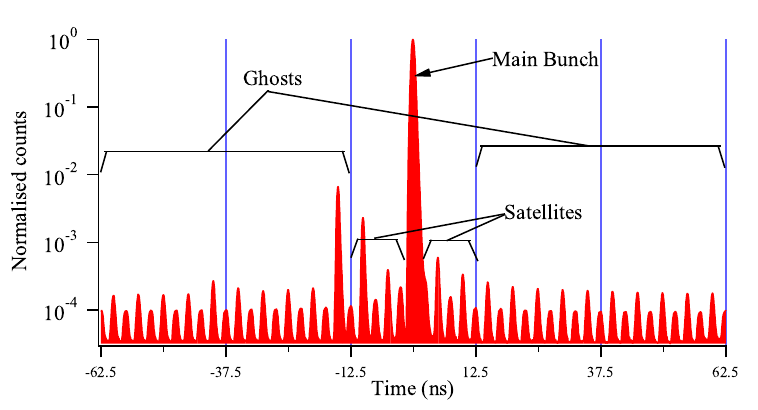
\includegraphics[width=4.5in]{/home/tensr/Dropbox/PHD_Thesis_HEP/PHD_THESIS/PHD/THESISPLOTS/Ghost-Satellite-Bunches-LDM.png}} 
\captionof{figure}{Longitudinal Profile taken with LDM detector showing definition of Ghost/Satellite bunches with respect to main bunches.}
\label{fig:LDM-Ghost}
\end{center}
The presence of ghost/satellite bunches increase the uncertainty in LHC luminosity measurements and can also generate proton-proton interactions in the collision region. Effects on ghost/satellite bunches on instantaneous luminosity measurements have been studied by both CMS, ATLAS and ALICE detectors \cite{ATLAST-GHOST} 
with their profile compared to main bunch bunches. CMS uses energy deposits in the endcap calorimeters with time space equivalent to those of ghost/satellite bunches while in ATLAS, they have also introduced a new detector called the Longitudinal Density Monitor~(LDM) to study ghost/satellite bunches. The results are shown in the figure \eqref{fig:CMS-ATLAS-Ghost}.
\begin{center}
\centering
\mbox{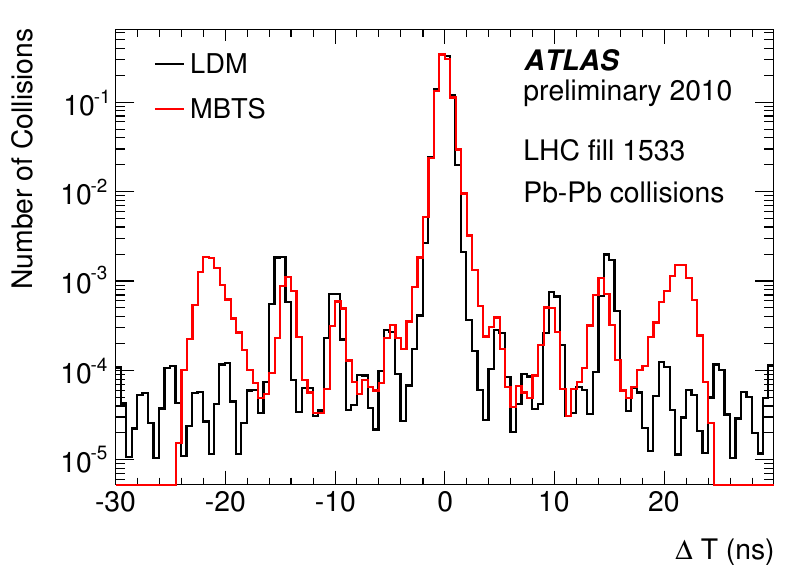
\includegraphics[height=2.5in,width=2.5in]{THESISPLOTS/ATLAS-LDM-GHOST.png} \quad \quad
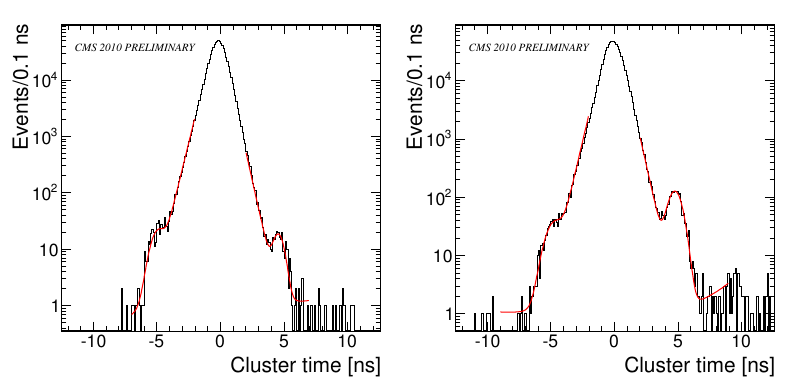
\includegraphics[height=2.5in,width=3.0in]{THESISPLOTS/CMS-Ghost-Profile.png}} 
\captionof{figure}{(left) Arrival time distribution(red) of ATLAS MBTS  for LHC fill 1533 during 2010 Pb-Pb run and LDM profile(black) for Beam2(same for Beam1).\newline
(Right) Timing of Clusters in the CMS endcap calorimeters for fill 1089:Left: EEP detector(left side of IP $z< 0$) Right: EEM detector( right side of IP, $z>0$). NB: Plots taken from \cite{ATLAS-GHOST} and \cite{CMS-GHOST}}
\label{fig:CMS-ATLAS-Ghost}
\end{center}
There is the possibility that ghost/satellite - ghost/satellite and ghost - Beam1/Beam2 collisions will happen generating events at the CMS detector. This is a major background in the search for delayed photons or objects in general as these collisions can occur \textit{in-time}(Beam1- Beam2) collisions or \textit{out-of-time} collisions. It is thus imperative to be able to quantify this contributions in any search analysis. We will show in future studies we have performs to both \textit{"guestimate"} and quantify these contributions in our search analysis.
\paragraph*{Beam Halo}\mbox{}\\
In addition to ghost/satellite bunches generating collisions events during collision, protons in ghost/satellite bunches can interact with collimators or gases such as H2, $CO_{2}$ and others in the beam pipe leading to the production of high energy muons which later bremsstrahlung and shower directly in the calorimeter detectors. 
Main bunches due to betatron oscillations(departure of particles from nominal orbit in the transverse direction) can also through inelastic scattering with gas molecules in beam pipe about 550~m up from interaction  point~(IP)(since beam cleaning in not being 100\% efficient), scattering on tertiary collimators~(TCT) about $z = 150$~m from IP and beam dump at about 150~m upstream CMS detector, produce through cascade decay energetic muons(sometimes muons with about 1~\TeV) which bremsstrahlung in calorimeter detectors. 

This kind of background from beam is referred to as \textit{Machine Induced Background}~(MIB) or \textit{Beam-Induced Background}~(BIB) and its contribution is called non-collision backgrounds as these are events observed in the detectors but not produced from the interaction point~(IP). Throughout these thesis, we will refer to this kind of events as \textit{Beam Halos or halos}. Because, they produce very high transverse momentum photons which can also be miss-identified as jets arriving in-time of out-of-time, they are a very important background in any analysis. In the later section, we will also show how we have developed new methods to identify and reject these kind of events and estimate its possible contribution to our analysis.


\section{Compact Muon Solenoid}
\subsection{Overview}
The goal of the  Compact Muon Solenoid~(CMS) detector is to identify particles by measuring their energies, momenta and track if applicable, as they pass through the detector. It is for this reason that the CMS apparatus is a general purpose particle detector operating about 330 feet underground at  point 5~(P5)LHC in cessy,France. Its main feature is a superconducting solenoid of 6~m internal diameter providing a field of 3.8~T necessary for good momentum resolution. 
This field  encloses and all-silicon pixel serving as a vertex detector and a strip tracker for charged particle track reconstruction, a lead-tungstate scintillating-crystals electromagnetic calorimeter (ECAL) and a brass-scintillating sampling hadron calorimeter (HCAL). Very long lived particles like muons are measured in gas-ionization detectors embedded in the flux-return iron-yoke located at the outermost section of the detector.
It has a simple cylindrical structure consisting of barrel and endcap detectors and an extensive forward calorimetry and detectors to provide a near $4\pi$ solid angle assuring good hermetic coverage
The CMS apparatus has an overall length of 21.6~m, a diameter of 14.6~m, and weighs 12,500 tonnes. 
\begin{center}
\centering
\mbox{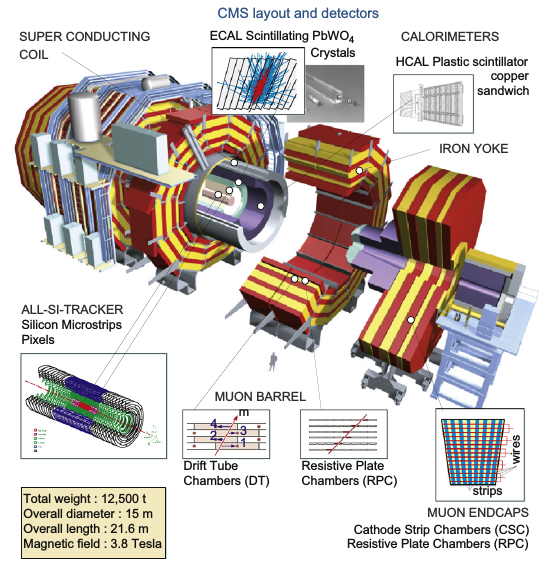
\includegraphics[width=10cm]{THESISPLOTS/CMS_LAYOUT_AND_DETECTORS.png}} 
\captionof{figure}{CMS Detector showing the different subdetectors and their material.}
\label{fig:CMS-DET}
\end{center}
The CMS detector performance can be summarised as seen in table \eqref{CMSRES} with the material type in each sub-detector.

\begin{center}\label{CMSRES}
\centering
 %\setlength{\abovecaptionskip}{0pt}
  %\setlength{\belowcaptionskip}{10pt}
 % \topcaption{GMSB,GGM Phenomenology and Relevant final states}
  \begin{tabular}{|l|l|p{3.2cm}|p{3.9cm}|}
  \hline \hline
  \multicolumn{4}{|c|}{\bfseries{CMS Detector and Resolution}} \\
  \hline \hline
  \bfseries{Subdetector} & \bfseries{Quantity} & \bfseries{Resolution} & \bfseries{Uses}  \\
   \hline \hline
 Tracker   & Momentum[GeV/c]  & $\sigma_{T}/p_{T} \approx 1.5\times 10^{-4}p_{T} + 0.005$ & \mbox{Silicon Pixels and Strips} \\ 
  \hline
  ECAL   & Energy[GeV] & $\sigma/E \approx 3\% /E + 0.003$ & $\pb$ Crystals \\
   ECAL  & Time[ns] & $\sigma(\Delta t)= \frac{N}{A_{eff}/\sigma_{n}}\oplus\sqrt{2}\bar{C} $ & $\pb$ Crystals \\
  \hline
  HCAL & Energy[GeV] & $\sigma/E \approx 100\% /E + 0.05$ & Brass + Scintilator\\
  \hline
  Muon Chambers & Momentum[GeV/c] & $\sigma_{T}/p_{T} \approx$ 1\%  \@ 50 GeV to  10\% \@ 1 \TeV & inner tracker + Muon Systems \\
  \hline
  Magnetic field & B-field strength[T] & 3.8~T + 2~T & Solenoid + Return Yoke\\
  \hline
  Triggers  & On/Off-line & Levels &\mbox{L1(On-line)} +\mbox{HLT(Off-line)}(L2+L3) \\
  \hline
  \hline
  \end{tabular}
  \captionof{table}{CMS Detector Material and Resolution(Time resolution: $N\approx 35$~ns, $\bar{C}\approx 0.020$~ns \cite{Time})}
 \label{tableCMS}
 \end{center}

The CMS uses a coordinate system where the origin coincides with the center of the detector also known as the nominal collision or interaction point~(IP). The direction of $x,y,$ and $z$-axis with the $z$-axis pointing towards the Jura Mountains from P5 are shown in figure \eqref{CMSCORD}. A more convenient coordinate system used in expressing quantities of particles is the polar coordinates. Here, the CMS  uses the azimuthal angle $phi$ measured from the $x-y$ plane with $\phi = 0 $ being the $x$-axis and $\phi = \pi/2 $ the $y$-axis. The radial distance in this plane is denoted $R$ and the polar angle $theta$  measured from the $z$-axis is related to the \textit{pseudo-rapidity}, $\eta$ through the relation: $$\displaystyle{\eta = -\ln \tan(\frac{\theta} {2}) } $$. The co-ordinate system $(\eta, \phi, z)$ and its radial distance $R$ defines a point in the CMS detector whose volume is a cylinder. 
\begin{center}\label{CMSCORD}
\centering
\mbox{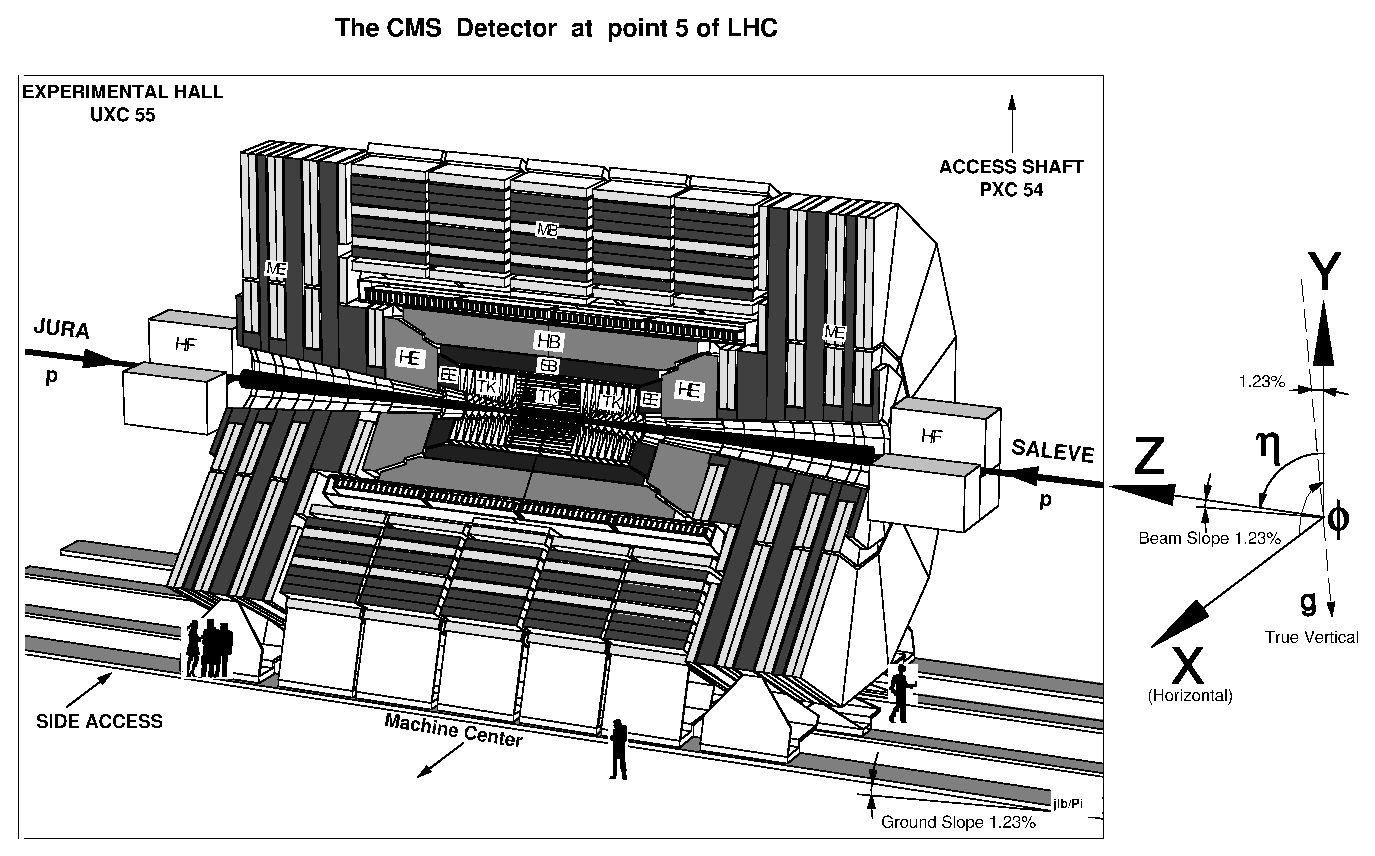
\includegraphics[scale=0.6]{THESISPLOTS/CMS_DETECTOR.eps}} 
\captionof{figure}{Schematic diagram of CMS detector view showing definition of cordinates as used by CMS.}
\label{fig:CMSDCORD.}
\end{center}

In CMS, quantities such as \textit{transverse momentum}~($p_{T}$), \textit{transverse energy}~($E_{T}$) and \textit{transverse missing energy}~($\MET$ or MET ) are used to distinguish a particle's quantities in the transverse plane($x-y$ coordinate) from those along the longitudinal direction($z$ coordinate) or beam line. In addition to these transverse quantities, cone-like structure with the cone radius is defined as $$\displaystyle{ \Delta R = \sqrt{ \Delta\eta^{2} + \Delta\phi^{2} } }$$ are used to measure the distance between two objects in the $\eta-\phi$ plane. These cone-like structures are used for particle isolation and identification purposes. In the next sections, we describe the characteristics and functionality of each of the CMS subdetectors introducing some additional details for those used in our analysis.


\subsection{Tracker}
Particles produced from proton-proton collision traverse the tracker sub-detector first. The job of the tracker is to measure the trajectory of charged particles, which are curved because of the magnetic filed produced by the magnetic coils. By measuring the curvature of these particle, the particle's momentum can be measured and its charge determined. The tracker is a silicon based detector and thus operates under the concept of ionization. It occupies a volume of 2.4~m in diameter and 5.4~m in length, consisting of pixel and strip sections geometrically arrange in cylindrical layers of barrel and disc-shaped endcaps, enclosed within the calorimeters. These sub-detectors all sit inside the 6~m in diameter solenoid magnet operating at 3.8~T. Figure \eqref{fig:CMSTRAK} depicts a schematic picture of the tracker with three barrel layers covering a region of radius from 4~cm to 15~cm in radius and two endcap discs within 49~cm on either side of the collision point along the $z$ axis; ten barrels layers  and twelve endcap disks per side of silicon strip detectors covering a region with radius from 15 to 110~cm and within 280~cm on either side of the LHC beam axis. The total tracker acceptance region in pseudo-rapidity is $|\eta| < 2.5$. The pixel detector is used for identifying the primary and secondary vertices of particles while the inner tracker of strip detector is for tracker reconstruction. 
\begin{center}\label{CMSTRAK}
\centering
\mbox{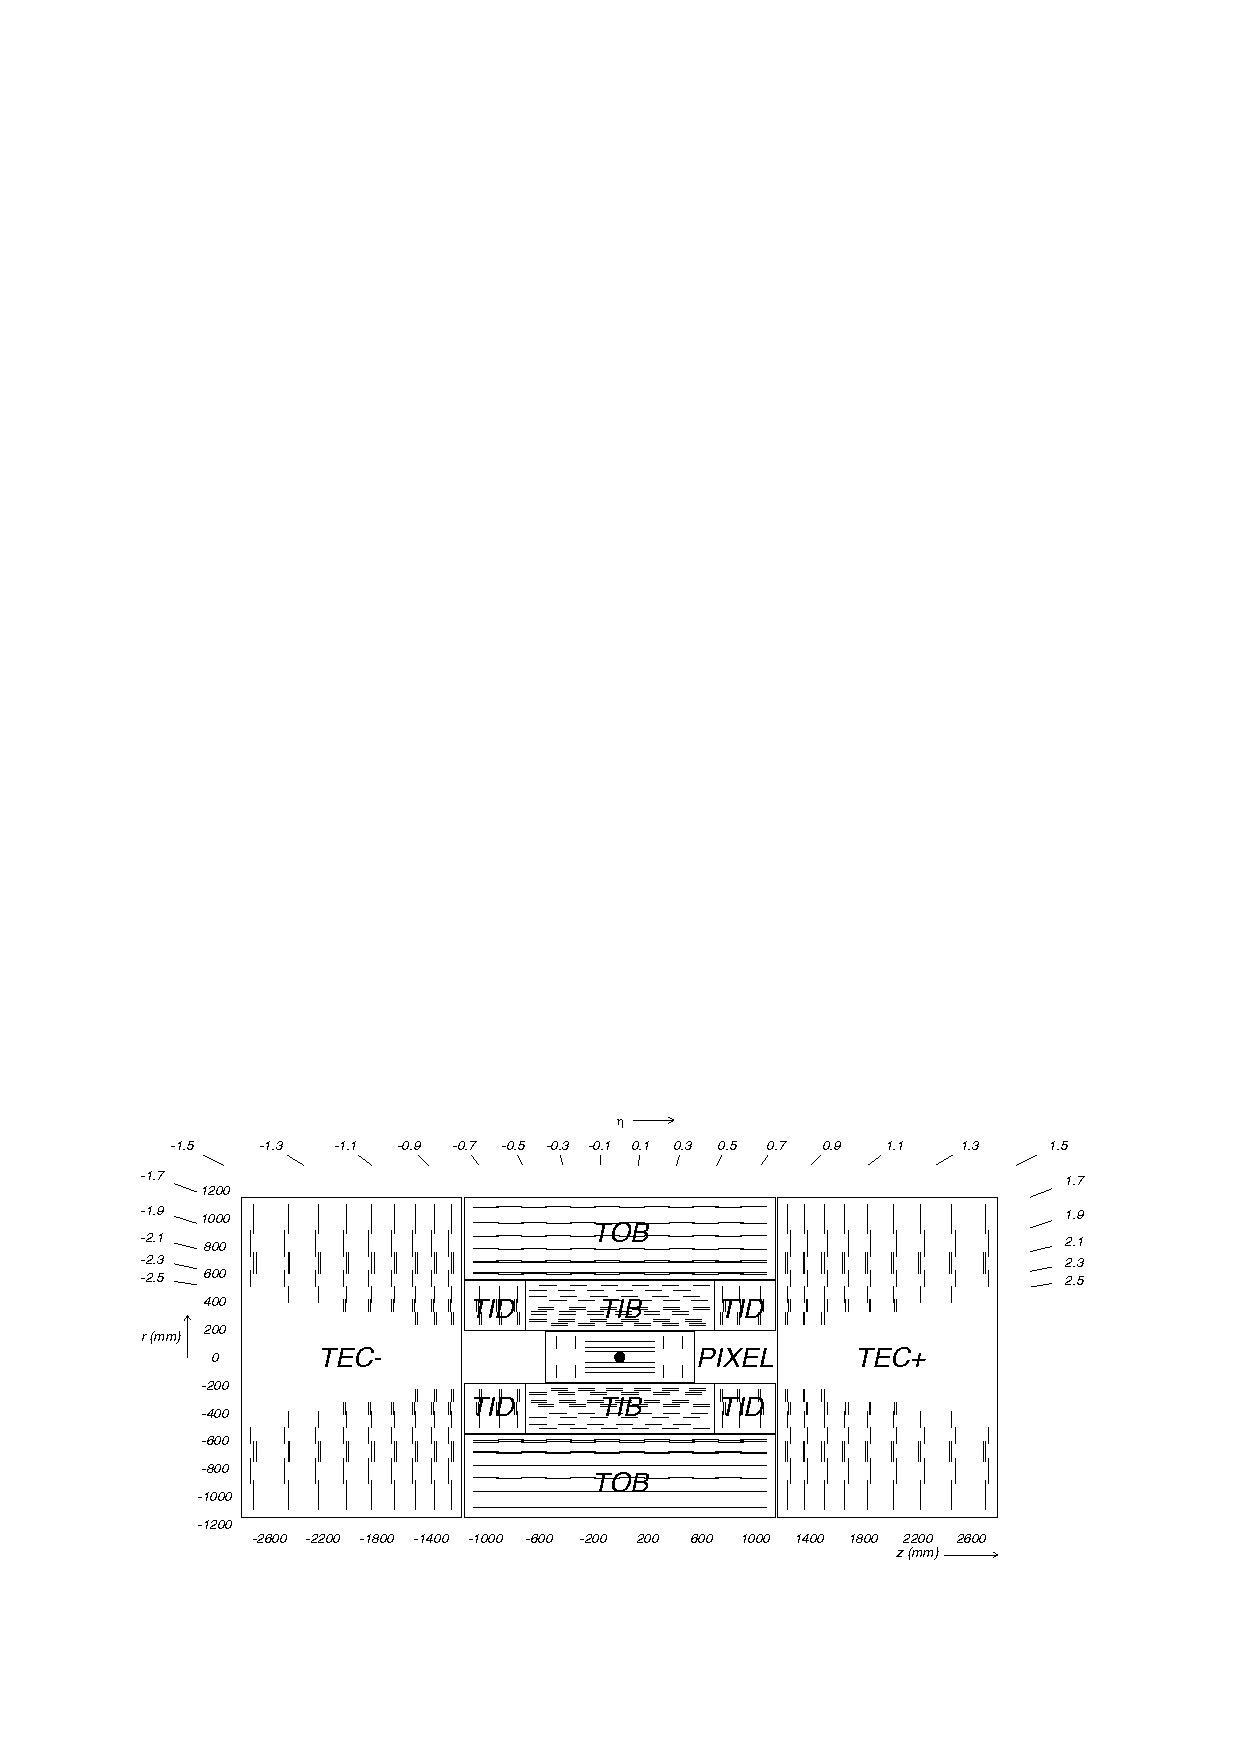
\includegraphics[scale=0.6]{THESISPLOTS/Tracker.pdf}} 
\captionof{figure}{Schematic diagram of CMS Tracker showing the silicon pixel detector region~(inner closer to LHC beam) and silicon strip reigion~(outer).}
\label{fig:CMSTRAK}
\end{center}
\subsubsection{Pixel}
The pixel vertex detector occupies the inner most region, very closed to the interaction region. Providing high-resolution and three-dimensional patterns of space points using silicon pads as pixels, the primary vertex and secondary vertices arising from the decay of heavy and relatively long-lived particles such as B-mesons containing b-quarks can be identified. This is also known as impact parameter measurements. The pixel covering a region of pseudo-rapidity $|\eta| < 2.4$ compliments the track finding by providing additional space points to seeding hits in the inner tracker.  Each pixel has a size of $100\times150$~$\mu m^2$ 
covering a total area of $\approx 1~m^{2}$ and there are 66 million pixels read out by 16000 readout chips on the silicon sensors. The pixel is organised in three 53~cm long barrel layers~(Pixel Barrel=PXB), positioned at radii  of 4.4, 7.3 and 10.2~cm and two disks each per side (Pixel Forward=PXF), placed at $\pm 34.5$~cm and $\pm46.5$~cm from the interaction point and covering a radii between 6 and 15~cm. This guarantees each charged particle track crosses at least two layers of pixels.
This arrangement ensures that the pixel detector provides  precise tracking points in the $ r-\phi$ and $z$ responsible for small impact parameter resolution of about $\sim 15~\mu m$. Small impact parameter resolution is important for precise secondary vertex  reconstruction and position resolution crucial in the identification of objects produced with displaced vertices with life-time of  about $\tau \approx 10^{-12}~s$ like mesons such as $B^{0,{\pm}}$, $D^{0,{\pm}}$, $\tau^{\pm}$, which may travel a distinguishable distance (c$\tau$ $\approx 100~\mu$m before decaying. Because of very high radiation dose of about 100~Mrad absorbed by the pixel detector, there is currently upgrade of the complete pixel detector in preparation of LHC Run 2.

\subsubsection{Silicon Strip Tracker}
CMS silicon inner tracker surrounding the pixel detector allows for the tracks of promptly produced charged particles with $\PT = 100GeV/c$ to be reconstructed with a resolution in the transverse momentum \PT  of about $\sim 1.5\,\%$. High momentum particles are less curved by the magnetic field than low momentum particles. Therefore, the tracker works complimentary with the calorimeter and muon detectors to ensure improve momentum resolution at all particle energies.
The silicon micro strip tracker covers a tracking volume up to radius of 1.2~m with a length of 5.6~m. It is organised in three parts: The inner tracker with four barrel layers (Tracker Inner Barrel=TIB) and three disks per endcap~(Tracker Inner Disks=TID), 6 outer barrel layers~(Tracker Outer Barrel=TOB) closed by 9 wheels on both sides.~(Tracker EndCap=TEC). 
The silicon strip is made of 15148 silicon microstrip detector modules. Each module has a set of sensors. It occupies an active area of $200~m^{2}$ providing a coverage in pseudo-rapidity up to
 $|\eta| < 2.5 $.
 The TIB/TID delivers up to 4 $r-\phi$ measurements on a trajectory using 320~$\mu$m thick silicon micro strip sensors arranged  parallel to the beam direction in the barrel and radial on the disks. The strip pitch is 80~$\mu$m on layer 1 and 2 and 120~$\mu$m on layer 3 and 4 of the TIB, leading to a single point resolution of 23~$\mu$m and 35~$\mu$m, respectively. The TID also have varying pitches with both the TIB/TID enclosed by the TOB. The layering structure can be seen figure \eqref{CMSTRAK}. The nearly 9.6 million silicon strips provide a spatial resolution measured to be about $10~\mu$m for $r-\phi$ measurement and about $20~\mu$m for $z$ measurement necessary for particle trajectory reconstruction.
 The combined pixel and micro strip modules allows for nearly 75 million readout electronic channels in the tracker.
 

\subsection{Calorimeter}
A calorimeter is a device which absorbs a good fraction of energy of an incident particle and produces a signal with an amplitude proportional to the energy absorbed. This absorption is via a cascade production of secondary particles where the incident energy is directly proportional to the number of secondary particles. CMS uses two types of calorimeters: Electromagnetic calorimeters~(ECAL) for absorbing the energy of electromagnetic particles such as photons and electrons and a sampling calorimeter or Hadronic calorimeter~(HCAL) made of more than one type of material for absorbing the energy of hadrons such as kaons and pions through hadronic interactions. The combined calorimeter detectors of CMS covers a region in $|\eta| < 5 $ making it nearly hermitic for missing energy measurements. The ECAL and HCAL are arranged in a layered manner as seen in figure \eqref{ECAL-HCAL} such that electromagnetic particles can be distinguished from hadronic particles by comparing the depth of the particle shower penetration in both calorimeters.

\begin{center}\label{ECAL-HCAL}
\centering
\mbox{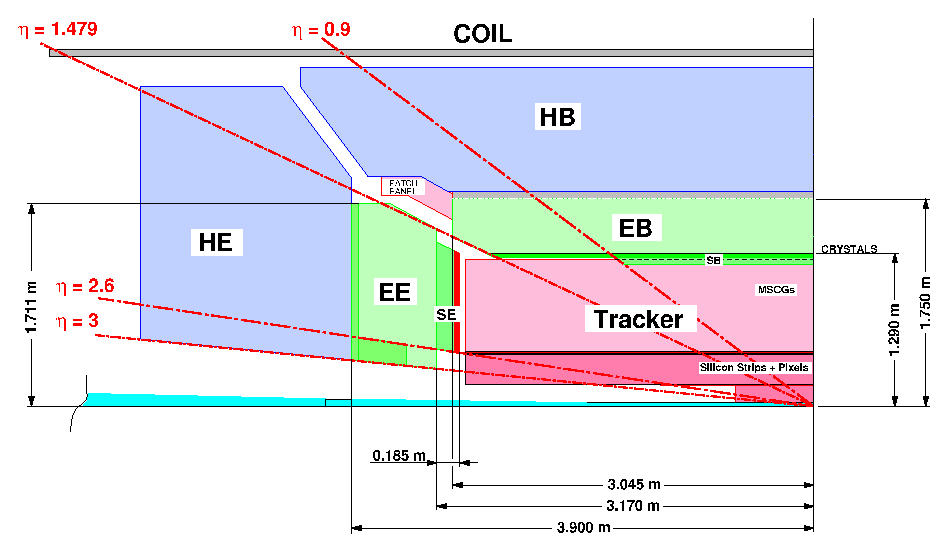
\includegraphics[scale=0.5]{THESISPLOTS/ECAL-HCAL.eps}} 
\captionof{figure}{Schematic diagram of CMS calorimetry system with HCAL enclosing ECAL in the Barrel and Endcap regions.}
\label{fig:ECAL-HCAL}
\end{center}

\subsubsection{Electromagnetic Calorimeter}
 The main particles to detect using ECAL detectors are photons and electrons. High energy photons and electrons are detected through their interaction with the material of the ECAL detector. During this interaction which can be either through electromagnetic showering also known as \textit{bremsstrahlung} or electron-positron pair production, the incoming photons or electrons deposit practically almost all of their energy. The material for the CMS ECAL detector are lead-tungstate~(\pb) crystals. There are 75848 lead-tungstate ~(\pb) crystals mounted in a barrel~(\textsc{EB}) and endcap~(\textsc{EE}) structure.   
 % The choice of \pb is due to its high density which allows for fast scintillating time of nearly 18~ns, has a fine granularity to enhance good resolution and is radiation resistant which are important characteristics in an LHC environment.
\pb crystal is the appropriate choice for calorimetry by CMS for operation in the LHC environment because of its a high density~(8.28~$g/cm^{3}$), short radiation length~($X_{0}$=0.89~cm) and a small Moli$\grave{e}$re radius~(22~cm). This dense nature allows for the electromagnetic shower to develop early and therefore very likely to be fully contained within a compact device.  In a high radiation dose and fast timing~(25~ns bunch spacing) environment like the LHC, the choice of \pb crystals is justified because of their high radiation resistance and short scintillation decay time of the same order of magnitude as the LHC bunch crossing time:about 80\% of the light is emitted in 25~ns.
Since the `amplitude'' or ``probability'' of a high energy photon or electron interacting with an ECAL material through (\emph{Bremsstrahlung}) and pair production is proportional to the nuclear charge or number of electrons, \text{Z} of the material, \pb which is a high \text{Z} material is once again CMS preferred choice for calorimetry. The small Moli$\grave{e}$re radius of \pb crystals ensures that on average about $95$\,\% of the electromagnetic shower energy is contained within the crystal volume therefore reducing the transverse spread of the electromagnetic cascade arising from multiple scattering of electrons. This improves on the estimation of the transverse position of impact of the incident particle and the fine granularity provides good precision for measuring the energy of an incoming electromagnetic particle and thus better energy resolution. 
 
The barrel section of the ECAL covers a pseudo-rapidity of $\vert \eta \vert< 1.479 $. The EB has 61,200 crystals providing a granularity of 360-fold in $\phi$ and $(2 \times 85)$-fold in $\eta$.The crystals are mounted in a quasi-projective geometry to avoid cracks aligned with a particle trajectories, so that their axes make an angle of 3\% with respect to a line vector from the nominal interaction vertex in $\eta$ and $phi$ directions. These EB crystals have approximately 0.0174~$\times$~0.0174  in $\eta-\phi$ or 22~$\times$ 22~$mm^{2}$ at the front face and 26~$\times$~26~$mm^{2}$ on the rear face. each crystal is 230~mm long corresponding to about 25.8~$X_{0}$ radiation length. The crystals are contained in a thin-walled aveolar structure made with aluminium called submodule with their radial distance from the center of the face of the crystals to the beam line is 1.29~m. Each submodule are arranged into 4 modules of different types according to their $\eta$ position with each module having about 400 to 500 crystals.  The four modules make one supermodule containing 1700 crystals. The aluminium surface is coated to avid oxidation hence coloration which causes decrease in transparency.  On the rear end of each EB crystals, is glued two Avalanche Photodiodes~(APD) whose purpose is to collect the scintillating light from the crystals converting light into current which is further collected by the read-out electronics.
 \newline
The endcap sector occupy a pseudo-rapidity region of 
$1.479 <\vert \eta \vert < 3.0$ with Preshower~(\textsc{ES}) detector made of silicon strip sensors interleaved by lead placed immediately in front of it.  The purpose of the preshower detactor is to help separate converted from unvonverted photons. There are two endcaps located in the $+z$ side of the nominal interaction and denoted \textsc{EE}$+$ and on the $-z$ side denoted as \textsc{EE}$-$. The longitudinal distance between the nominal interaction point and the center of the surface of the crystals in \textsc{EE} is 3.154~cm. Crystals in the \textsc{EE} are of identical shape group in  units of 5~$\times$~5 crystals called \textit{supercrystals or SC}. Each endcap is divided into two halves called \textit{Dees} with each Dee holding 3662 crystals. The crystals are arranged in $x-y$ grid with their front face and rear cross section of 28.62~$\times$~28.62~$mm^{2}$ and 30~$\times$~30~$mm^{2}$ respectively. Ecah crystal is 220~mm~(24.7~$X_{o}$) in length. Vacuum Phototriodes~(VPT) is glued on the rear face of each crystal for scintillating light collecting and conversion into electrical signals. These photodiodes and triodes are used because of their high gain and the fact that they are not affected by the high magnetic field. 
Although the light-yield for \pb is rather low~($\approx 70$photons/\MeV), the photodiodes have internal gain~($50$ for APDs and 10 for VPTs) and good quantum efficiency
of $75$\,\% for APDs and $20$\,\% for VPTs of the emission wavelength. This makes it possible that signals 
from incident particles with energies from a few to high \GeV can be recorded.
APDs and VPTs are the standard choice of photo-detectors by CMS because of their high resistance to radiation and smooth operation in a strong magnetic field environment. Photodiodes like APDs and VPTs are similar to silicon photodiodes, with the exception that they have a buried p-n junction reversed-biased at a very high electric field. The photo electrons arriving at the junction undergo avalanche multiplication giving the device a gain.
The signals from the APDs and VPTs are digitized by voltage-sensitive analogue-to-digital converters are later converted to light signals which are then transported using long optical fibres to the counting room located adjacent to the experimental cavern.
\newline
The energy resolution and geometric structure of the ECAL ensures that the photon or electron's arrival position at ECAL,energy and time and even the direction and shape of its electromagnetic shower in the crystals can be measured and identified respectively with good precision.

\begin{center}
\centering
\mbox{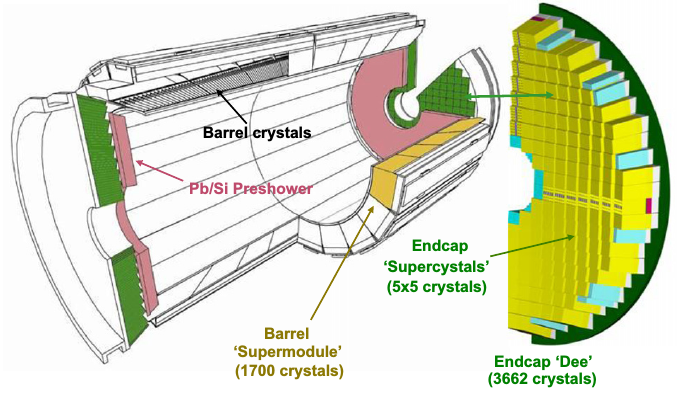
\includegraphics[scale=0.6]{THESISPLOTS/CMS-ECAL-EB-EE.png}}
%\mbox{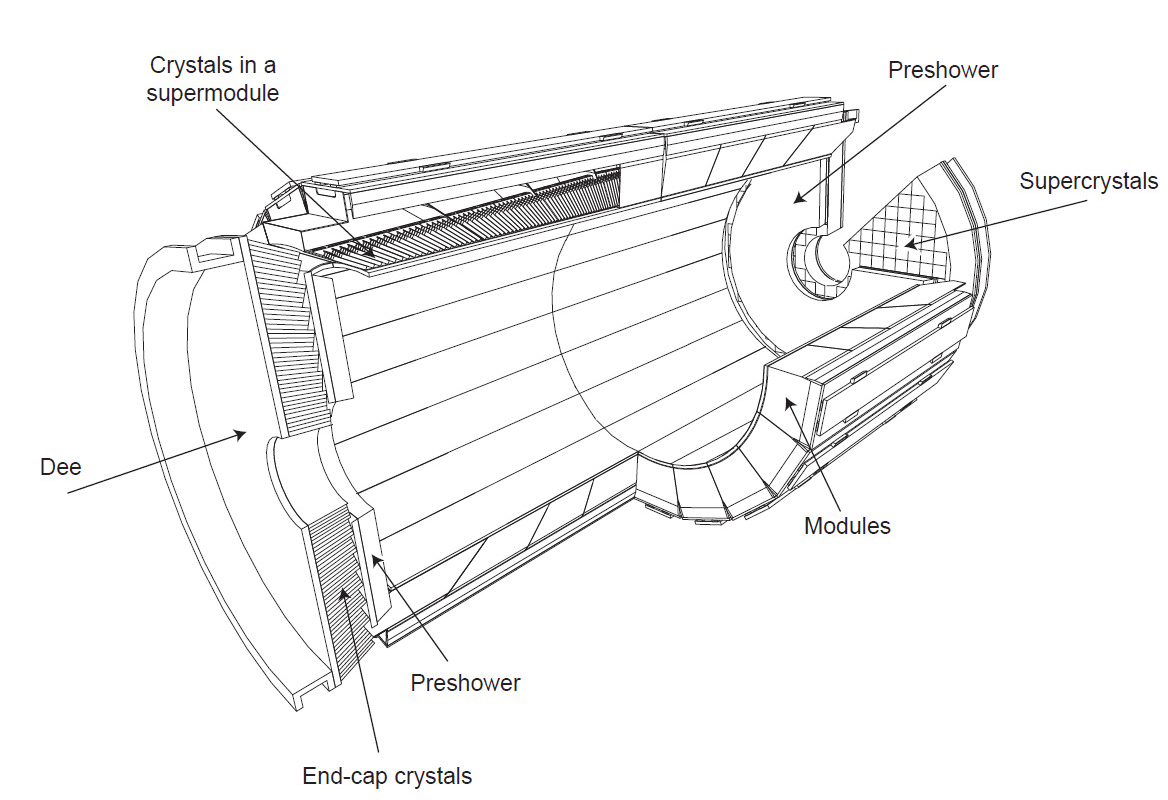
\includegraphics[scale=0.2]{THESISPLOTS/CMS-ECAL.png}}
%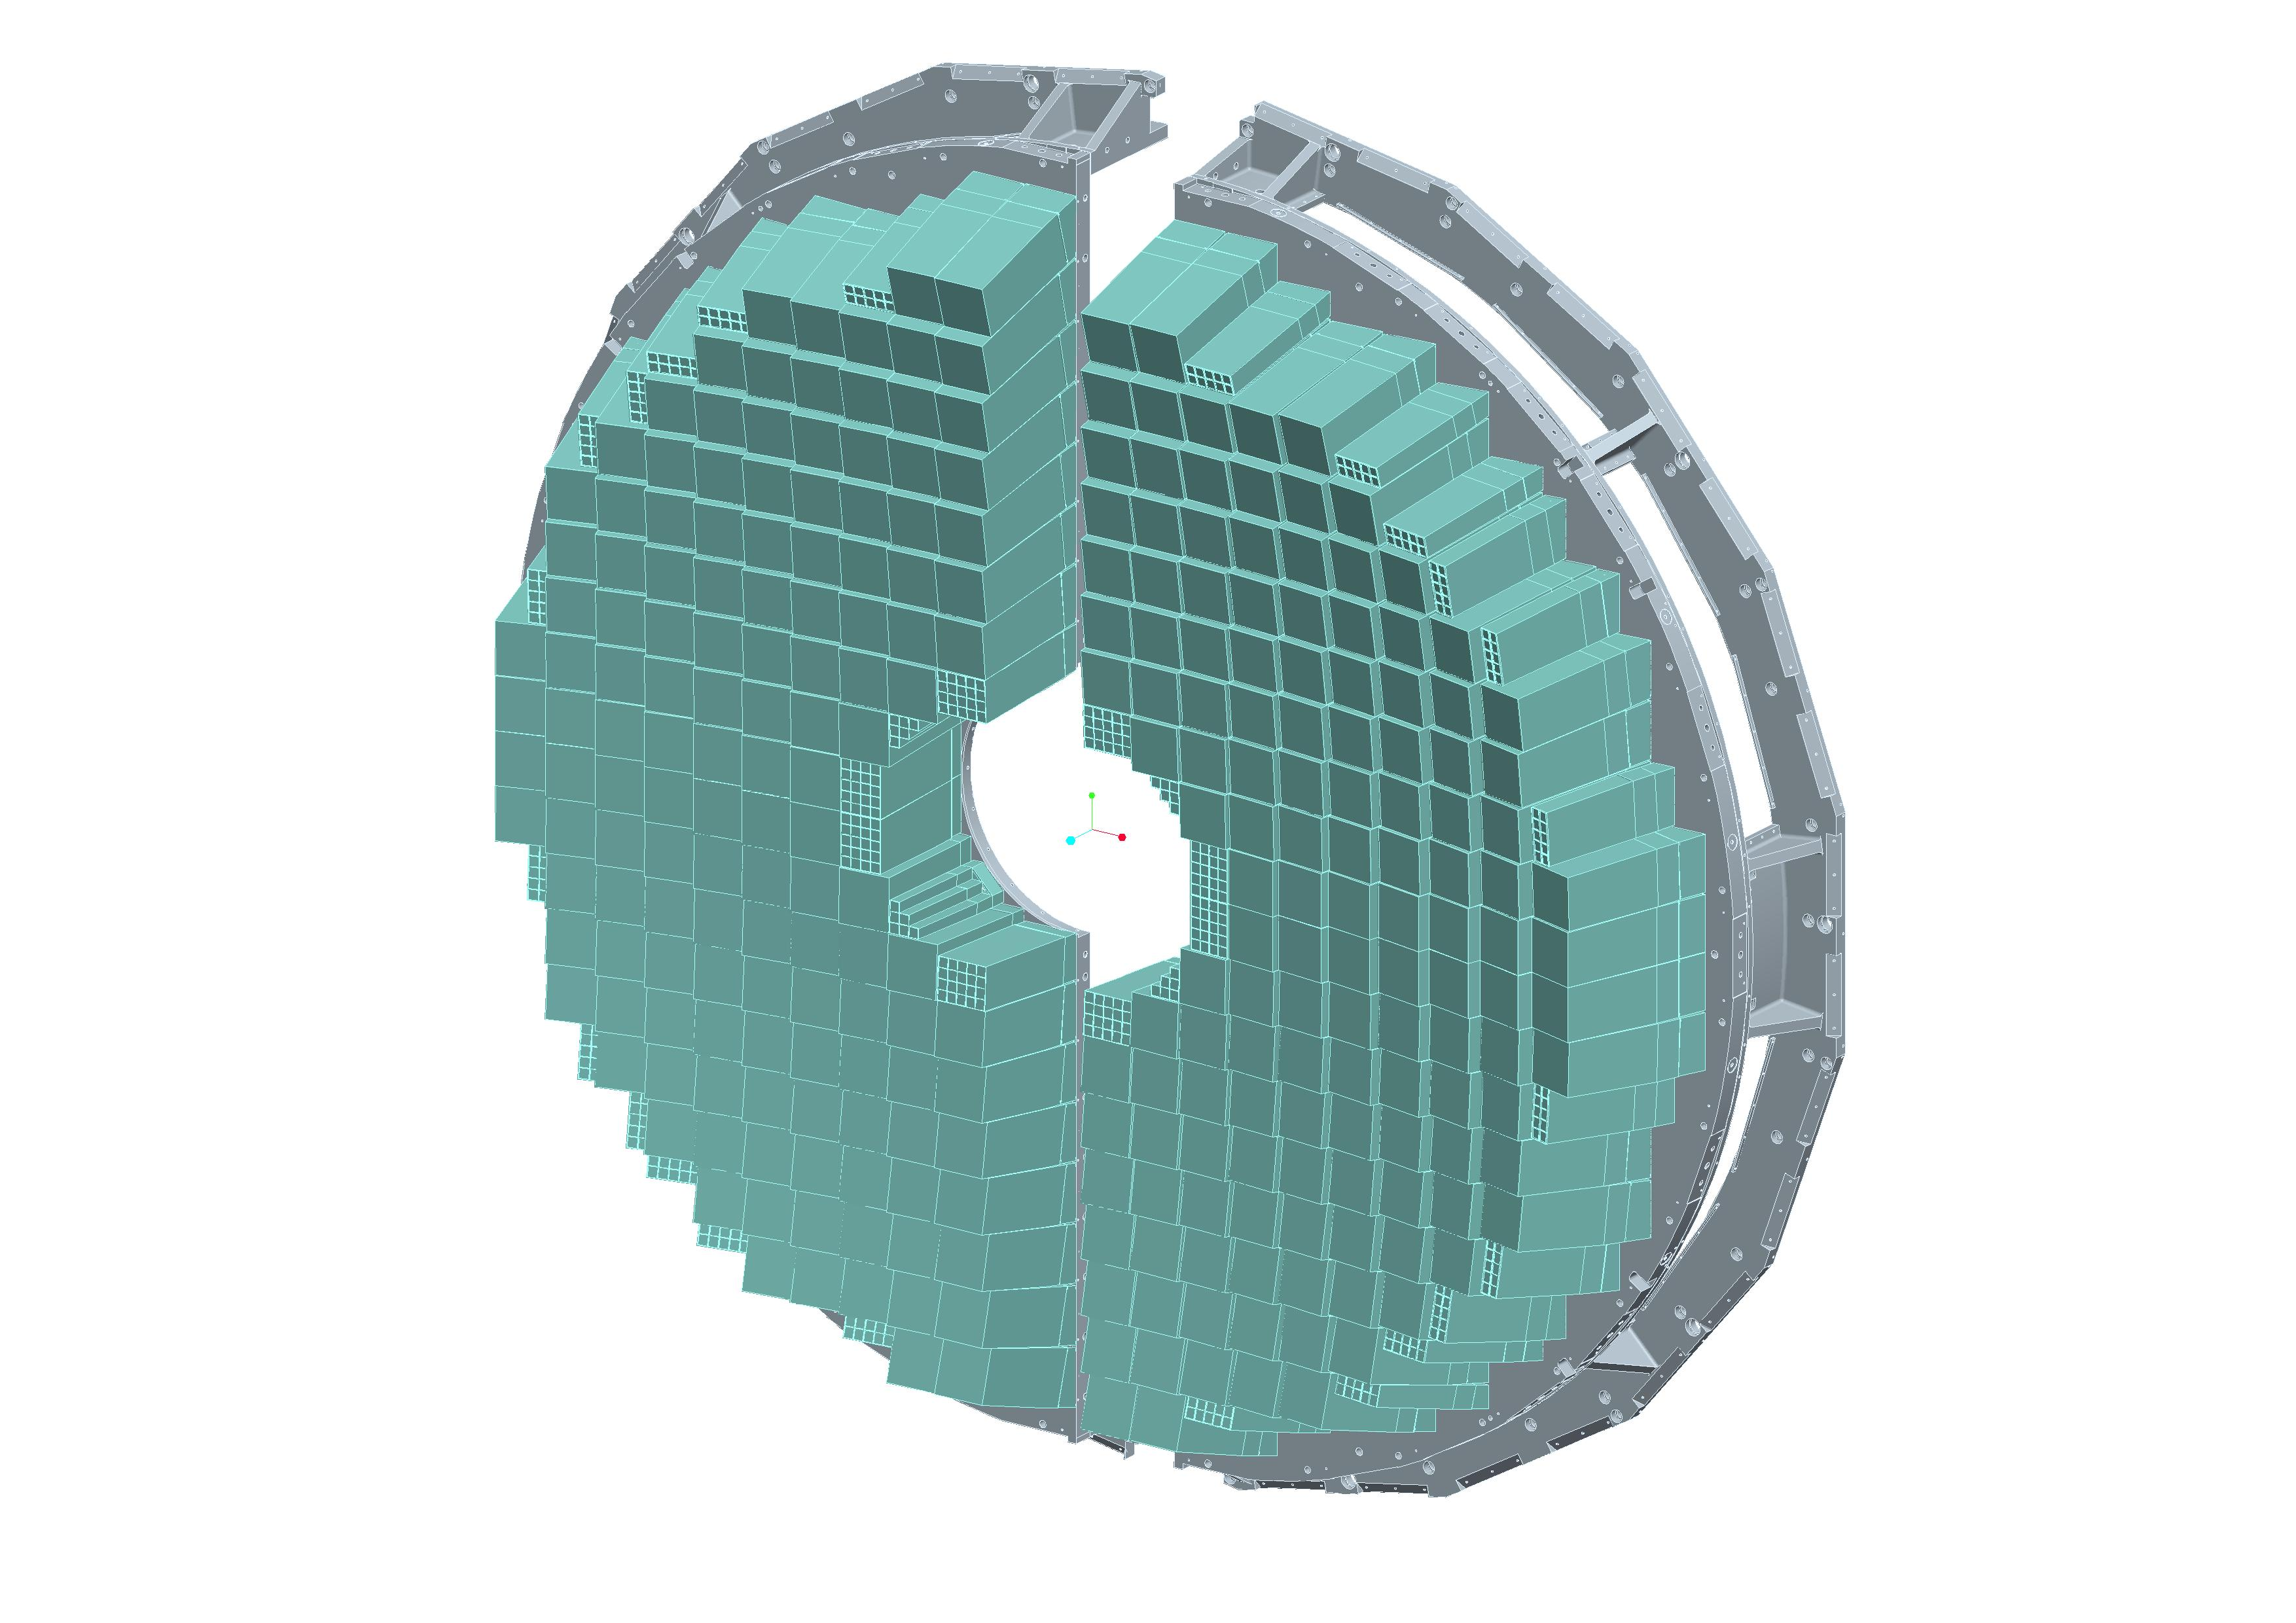
\includegraphics[scale=0.06]{THESISPLOTS/endcap_CMS.png}} 
\captionof{figure}{Layout of the CMS electromagnetic calorimeter showing the arrangement of crystal modules, supermodules in the barrel with the preshower infront of endcap with supercrystals.}
\label{fig:CMSECAL}
\end{center}






%This homogenous design of the ECAL provides it with a performance which is optimal(by design) in its potential to discover a Higgs in the mass region 
% less than $130$\GeV/$c^{2}$ through the decay $\displaystyle{H\rightarrow\gamma\gamma}$. 
% Homogenous design implies reduced noise in the detector  thus better resolution since only a single material type is in use.
%ECAL has a current  timing resolution better than 500~ps for large energy deposits(more than 10-20~GeV in the \text{EB})~\cite{TIME} 
%and an energy resolution of ${\displaystyle\sigma/E\approx 0.45\,\%}$ for unconverted photons with energies above 100~GeV~\cite{CMSTDR}.
 



\subsubsection{Hadronic Calorimeter}
Hadrons like protons, neutrons kaons and pions are unlike electromagnetic particle strongly interacting~(strong force is the force that binds nuclei together). A hadronic shower is formed when an incident hadron undergoes an inelastic collision with the nucleus of the absorber material producing secondary hadrons which as they go through successive layers of absorber material interact inelastically with other nuclei to produce further hadrons etc. 
The  hadronic cascade loses about 30\,\% of incident hadron energy through nuclear excitation of the nuclei of atoms of the  absorber material.  Hadronic showers start to develop later with more lateral spread and and larger in the longitudinal dimensions than electromagnetic showers. This is why the hadronic calorimeter~(HCAL) is made of alternating plates of brass and plastic scintillator encompassing the ECAL. The scintiallating light is readout using wavelength shifting optical fibres by photosensors in the barrel and endcap. The photosensors are hybrid photodiodes~(HPD). The are ongoing upgrades to replacing the HPDs with silicon photon multipliers~(SiPM). 
The  hadronic barrel(\text{HB}) and hadronic endcap(\text{HE}) of the HCAL cover a region in pseudo-rapidity of $\vert \eta \vert < 3$. While the Hadronic Forward~(\text{HF}) occupies a pseudo-rapidity region of $3 < \vert \eta \vert < 5$.
The HB calorimeter is an assembly of two half barrels each composed of 18 identical $20^{o}$ wedges in $\phi$. Each wedge is made of flat brass alloy absorber plate parallel to beam axis with the innermost and outermost layers made up of stainless steal interleaved by plastic scintillating tiles.
The first active layer is situated directly behind the ECAL in order to actively sample low energy showering particles from the support material between the ECAL and HCAL. Each scintillating tile has a size of $\Delta\eta\times\Delta\phi=0.087 \times\ 0.087$ and is instrumented with a single wave length shifting fiber(WLS) for better collection of light. The summed optical signals or light are converted into fast electronic
signals by photo-sensors called  hybrid photo-diode(HPD).
This inhomogeneous design gives the HCAL, an energy resolution of ${\displaystyle \Delta E/E \approx 0.5/\sqrt{E(GeV)} }$ for particles with energy above 250~GeV, much lower compared to that of homogeneous ECAL detector.

The forward hadronic~(HF) calorimeters placed upstream have scintillating tiles called Beam Scintillation Counters~(BSC) which in coincidence with the beam pick-up monitors ~(BPTX) detector helps to eliminate beam background contamination at the trigger level and is also useful for detection of hadrons in the forward region. HF made up of steel absorbers embedded in radiation hard quartz fibers running parallel to the 
beam axis and providing a fast collection of Cherenkov light. The signal results from Cherenkov light emitted in the quartz 
fibres embedded in the steel matrix in response to charged particles.
The Cherenkov calorimeter have long and short fibers which are positioned alternatively separated by 5~mm with readouts for better sampling of the different shower components.
The goal of this hardware design is to give better compensation for different shower components in the hadronic shower.
The HF section enables the HCAL to pick up myriad of particles coming out of the collision point. Quartz fibre has high resistance to the high radiation does in the forward detectors and light production is through Chererenkov method than scintillation in HB and HE calorimeters.
 
The purpose of the HF detector is to provide a full hermetic $4\pi$  phase space coverage required for missing transverse energy calculation or \text{MET}. MET is the established as signal for very weakly interacting particles like neutrino and supersymetric particles like gravitino which travel through the detector undetected.
For $\vert \eta \vert< 1.74$ region, the HCAL cells are $0.087 0.087$\,rad  in pseudo-rapidity($\eta$) and in azimuth ($\phi$).
In the $(\eta,\phi)$ plane, and for $\vert \eta \vert < 1.48$, 
the HCAL cells map on to $5 \times 5$ ECAL crystals arrays to form calorimeter towers projecting radially outwards from close 
to the nominal interaction point. At larger values of $\vert \eta \vert$, the size of the towers increases and the matching ECAL arrays contain fewer crystals. 
Within each tower, the energy deposits in ECAL and HCAL cells are summed to define the calorimeter tower energies subsequently used to provide the energy and direction. The ratio of the energy deposit if a particle in the ECAL crystals to that in the HCAL towers is used to distinguished between true photons from neutral hadronic showers.
% \newline
% All these information is fed into the PF algorithm for particle reconstruction.
\subsection{Muon Chambers}
Muons are long-lived particles capable of travelling across the entire lateral section of the CMS detector into the muon chambers producing tracks in the tracker and depositing very little fraction of their energy in the calorimeters. The muon chambers uses ionization and the magnetic field from the return iron yokes to curve the tracks of charged long-live particles like muons, measuring their momentum and finally detecting them. There are three different types of muon chambers: the drift tubes~(DT) chambers in the barrel, cathode strip chambers~(CSC) n the endcaps and resistive plate chambers ~(RPC) glued to the DT and CSC chambers. Four layers or stations of DT/RPC and CSC/RPC are embedded in an interleaved  style with the iron yoke for track reconstruction and triggering. Figure \eqref{cmslview} provides a longitudinal view of the CMS detector showing the position of the stations.
The DT and CSC record track segments characterised by the position of the track and the bending angle which is used to determine the precise transverse momentum and charge of a given particle during off-line reconstruction. The RPCs are dedicated trigger chambers used to determine the candidate muon's approximate transverse momentum ad bunch crossing number where the particle originates. The RPC has a timing resolution of about 3~ns.

%%%%%%%%%%%%%%%%%%%%%%%%%%%%%%%%%%%%%%%%%%%%%%%%%%%%%%%%%%%%%%%%%%%%%
\begin{center}\label{CMS-SUBD}
\centering
\mbox{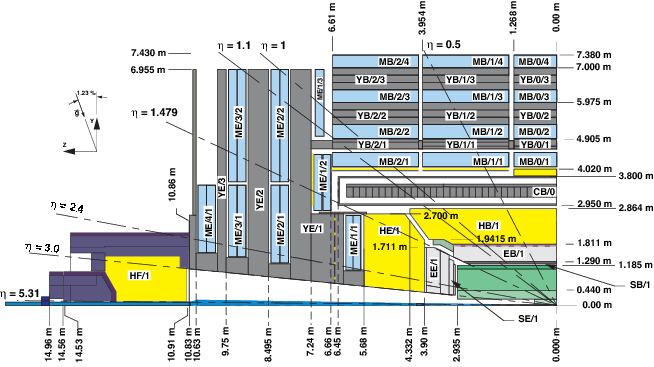
\includegraphics[scale=0.6]{THESISPLOTS/CMS_Int_View.png}} 
\captionof{figure}{Longitudinal view of CMS showing the coverage range of its sub-detectors.}
\label{fig:cmslview.}
\end{center}

\subsection{Particle Detection}
Particle types that are identified using the CMS detector include electrons, photons, hadrons, muons, neutrinos and other weakly interacting particles. These particles depending on their charge, nature of interaction and lifetime can be identified either using some or all the sub-detectors of the CMS detector.
The figure \eqref{cmsSLICE} show a  transverse slice of the CMS detectors with tracks in the tracker and muon sub-detectors and calorimeter energy deposit showing how different particles interact with the material in different sub-detectors thus ensuring their unique identification and reconstruction in the detector.

\begin{center}\label{CMSSLICE}
\centering
\mbox{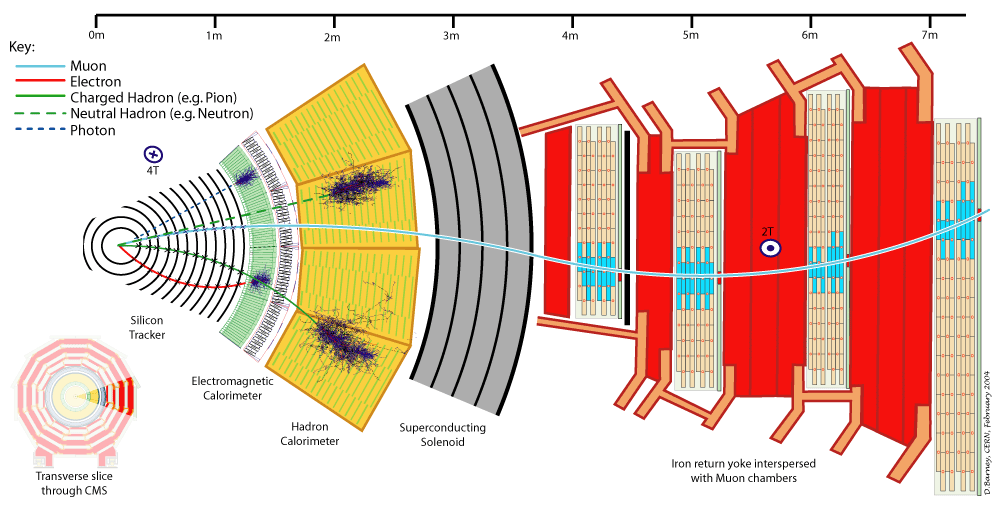
\includegraphics[scale=0.4]{THESISPLOTS/CMS_Slice.png}} 
\captionof{figure}{Transverse slice of the CMS detector showing how different types of particles interact and hence identified using this detector.}
\label{fig:cmsSLICE}
\end{center}


\subsection{Triggering}
In CMS, there are a billion interactions happening every second which means data from protons colliding 40 million times every second equivalent to the 25~ns LHC bunch crossing time interval has to be process and analyse before the next collision happens. Obviously this is impossible and infact, not every proton-proton collision will lead to the production of an interesting physics event. Thus one has to find a way of selecting only events produced from head-on proton collision with sufficient amount of energy. Even with this selection, it is not possible to process a single event in a 25~ns time frame. Thus, the CMS uses a two level triggering system for selecting interesting events and a pipeline system to temporarily store and process information from many interactions at the same time. Thus so as not to confuse particles from two different events, the CMS triggering system has a very good timing resolution and synchronization so that signals from millions of electronic channels and synchronised and identified to be produced by the same event.
The CMS triggering system consist of two layers: The Level-1~(L1) and High Level Triggers~(HLT) triggers. L1 triggers are hardware designed electronic system while HLT is a farm of more than 1000 standard computers running the HLT event selection algorithm. Thus event selection begins at the L1 and HLT triggers.
The L1 trigger electronics is implemented in FPGA and ASIC technology and consists of a calorimeter, muon trigger and a global trigger boards. The global trigger board makes the final decision based on the calorimeter and muon triggers to reject or keep and event for further processing at the HLT trigger. The L1 trigger is responsible for selecting the best 100,000 events each second from the initial 1 billions events from interactions happening every second. The pipeline system is used during the L1 trigger latency time of about 3.2~$\mu$s.
The HLT trigger using assimilated and synchronised information from different parts of the detectors recreates the entire event. the HLT runs complex algorithm relating to physics objects like matching tracks to hits from the muon chambers  or energy deposits above a certain threshold in the calorimeters without tracks for electromagnetic objects. By the time this selection process in complete, there are now only 100 events per second with the remaining 99,900 thrown away.
With the average event size of about 1~Megabyte, in a stable and effective LHC proton collision year or $10^{7}$~seconds, the CMS produces about a Petabyte of data which is stored in tapes for later offline analysis. Due to the large amount of data, such analysis are performed using clusters of computers geographically connected to each other in a virtual computing environment called the LHC Computing Grid~(LCG) to which the CMS is a member. This data is made available to 7 primary and later to secondary tier centres consisting of national research laboratories and universities around the world using a data transport system term Physics Experiment Data Export~(PhEDEx).
\label{Collider_And_Detector_chapter}
%%%%%%%%%%%%%%%%%%%%%%%%%%%%%%%%%%%%%%%%%%%%%%%%%%%%%%%%%%%%%%%%%%%%%%%%%%%%%%%%
